\section{The \emph{k}-medians problem}
The \emph{k}-medians problem is a variant of the k-centers problem 
which penalizes the sum over all distances, and not just the maximum distance
as in the k-centers problem.

\begin{enumerate}
\item \underline{Input}: a set $S$ of $n$ points $x_1,....x_n \in 
\mathcal{X}$ assuming $(\mathcal{X},\rho)$; a positive integer $k$
\item \underline{Output}: $T \subset \mathcal{S}$ s.t. $|T| = k$
\item \underline{Goal}: minimize the cost of $T$ where: $ cost(T)
:= \sum_{i \in \{1...n\}} \rho(x_i,T) $
\end{enumerate}

The problem is very similar in structure to the \emph{k}-centers problem,
but in the k-medians setting, the set of possible centers $T$ is restricted to the set of data points $S$,
and the cost function is a sum of distances over all data points instead of simply considering the maximum distance. 

\begin{remark}
The fact that k-medians considers a sum over all distances makes solutions to
this problem somewhat more robust to outliers than the \emph{k}-centers problem,
since a single outlier does not necessarily dominate the cost.
\end{remark}

\noindent\textbf{Relaxed Linear Programming Techniques:} Because the objective function for this problem is linear in the choice of
centers in $T\subset S$, it is susceptible to a modified linear programming strategy.\\

Let $0< i\leq |S|$ and $0 < j\leq |S|$ index the set $S$. Then define two
binary variables $y_j$ and $x_{ij}$ such that

$$y_j = \mathbbm{1}\left[j^\text{th}\text{ datapoint is in } T\right]$$
and
$$x_{ij} = \mathbbm{1}\left[i^\text{th} \text{ point is assigned to the cluster centered at the }j^\text{th} \text{ point}\right]$$

In other words, $y_j$ is a binary variable that asks if the 
$j^\text{th}$ point is a cluster center (i.e. an element of $T$), 
and $x_{ij}$ is a binary variable that asks if the nearest center to
the $i^\text{th}$ data point is the $j^\text{th}$ data point.

\begin{example}
	For example, consider three data points $S=\{0, 2, 3\}$ and
	$T=\{0, 2\}$. In this case, 0 is assigned to 0, 2 is assigned to 2, and 3 is assigned to 2,
	so $x_{00} = 1, x_{11}=1, x_{12}=1$ and all others are 0. $y_0$ and $y_1$ are 1, and $y_2$ is 0.
\end{example}

With these definitions, we can reformulate the k-medians problem as 
an integer programming problem minimizing the objective function

$$\min_{(x_{ij}, y_j)_{i, j \in \{1...n\}}} \sum_{ij} x_{ij}\rho(x_i, x_j)$$

subject to the constraints that
\begin{align}
	& \forall i \in \{1...n\}, \quad\sum_j x_{ij} = 1 \notag \\
	& \sum_j y_j = k \notag \\ 
	& \forall i, j \in \{1...n\},  \quad x_{ij} \leq y_j \notag \\
	& \forall i, j \in \{1...n\},  \quad x_{ij}\in \{0, 1\}, y_j\in\{0, 1\} \notag
\end{align}

This objective, while superficially different, is equivalent to the original problem, 
since the objective is minimizing the sum of indicator variables which reduces
to the original sum over the assigned centers. The first constraint requires that 
each datapoint be assigned to one and only one cluster center, while the second 
constraint requires that $|T|=k$. The third constraint forces the $i^\text{th}$ 
datapoint be assigned to the $j^\text{th}$ datapoint if and only if $x_j$ is in fact
a cluster center. The last constraints enforce the conditions that $y_j$ and $x_{ij}$
are binary variables. 

The first three groups of constraints are linear in $y_j$ and $x_{ij}$, but problematically, the last constraint is not.
It is in fact an integer constraint, making this an integer linear program (ILP). These problems are known to be NP-complete, making the problem intractable in general. However, that sole integer
constraint can be relaxed into a linear constraint by requiring only that

$$\forall i, j \in \{1...n\}, x_{ij}, y_j \in[0, 1]$$

This problem is now linear (in $n^2 + n$ variables) and can be solved with a typical linear program solver.

Now we want to compare the solutions from the integer linear program and the relaxed linear program. Suppose the optimal solution to the ILP has cost $OPT$, and the optimal solution to the LP has cost $OPT_{LP}$. Observe that $OPT \geq OPT_{LP}$ because the cost can only go down when we have more choices for the variables (in this case, more choices for $x_{ij}$ and $y_j$). \\

\newpage

\noindent\textbf{Pros and Cons of the Relaxation:} The relaxation makes this problem efficiently solvable. There are many methods for solving a linear program (the list is non-exclusive, meaning that there are overlaps between categories of methods):

\begin{itemize}
\item Simplex method: exponential time in worst case, but very good in practice.

\item Ellipsoid method: proposed by von Neumann, usually $O(n^6)$ where $n$ is the number of variables in the linear program.
\item Interior point method
\item Cutting-plane method
\item ``Branch and Bound": usually directly used for ILP.
\item Criss-cross method
\item Primal-dual method
\end{itemize}

Currently the best runtime is achieved by a special case of interior point methods: $O(n^{3.5})$ by Karmarkar's algorithm. \\

However, the con of relaxation is that the LP solution is fractional, so it is not an exact solution to the ILP. How can we resolve this? \\

\noindent\textbf{Two approaches to converting the LP solution to an ILP solution: }As hinted above, the solution obtained to the relaxed linear program can clearly violate the original $k$-medians criterion, because fractional assignments may occur. Two methods of rounding can remedy this issue. (i) We can simply round the LP solution and analyze the result. However, the approximation achieved by this na\"ive rounding can be arbitrarily bad. (ii) We might also try a randomized rounding, where variables in the ILP are assigned by flipping coins with biases that are the values of the corresponding variables in the LP. Still, it is possible that this method will return something that is not even in the solution set, although this occurs with very low probability. (Note that derandomization procedures are also available). This discussion leads us to the following algorithm:

\begin{algorithm}[H]
\caption{Deterministic polynomial-time algorithm for $k$-medians problem using linear programming relaxation}\label{kmedian}
\begin{algorithmic}
\STATE Run the linear program on inputs $S\subset \mathcal{X}$ and $k\in\mathbb{N}$
\STATE Define $c_i:=\sum_j x_{ij}\rho(i, j)$ $\forall i\in[n]$
\STATE \textbf{Note:} The linear program's optimal solution $OPT_{LP}=\sum_i c_i$
\STATE $T\leftarrow \varnothing$
\WHILE{$S\neq\varnothing$}
\STATE Pick $i$ with the smallest $c_i$
\STATE $T\leftarrow T\cup\{i\}$.
\STATE Define $A_i:=\{i'\in S\;|\; B(i,2c_i)\cap B(i', 2c_{i'})\neq\varnothing\}$
\STATE $S\leftarrow S\setminus A_i$
\ENDWHILE
\end{algorithmic}
\end{algorithm}

\begin{figure}[h]
\centering
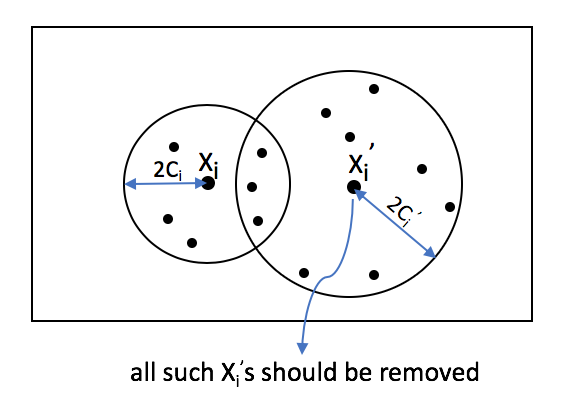
\includegraphics[width=0.7\textwidth]{chapter_1/files/kmedians_polytime_algo}
\caption{Visualize the deterministic poly-time algorithm. }
\end{figure}
\subsection*{Claim 1: COST(T) $\leq 4$ OPT$_{\text{LP}}$}
\subsubsection*{Observation:}
Pick any $q \in S$ and suppose $i$ is the first point selected in $T$  for which $q \in A_i$.

\begin{enumerate}
	\item $c_i \leq c_q$
	\item $\rho(q, i) \leq 4 c_q$
\end{enumerate}

\noindent\textbf{Proof:} \\
$$\exists p \in S, \rho(q, i) \leq \rho(q,p)+\rho(p, i)\leq 2c_q+2c_i \leq 4c_q$$ \\

\noindent Summing up both sides of the inequality over $q$, we get $COST(T) \leq 4 OPT_{LP}$.
\subsection*{Claim 2: $\mid$T$\mid$ $\leq 2k$} 
\subsubsection*{Observation:}
\noindent Pick any $i \in T$, we have:
$$k \geq \sum_{j \in \text{Ball}(i, 2c_i)}y_j \geq \sum_{j \in \text{Ball}(i, 2c_i)}x_{ij} \geq \frac{1}{2}$$

\noindent\textbf{Proof:} \\

\noindent Recall constraints when defining our linear program for $k$-median: \\
$$ k \geq \sum\limits_{j} y_j$$ (There are at most $k$ centers.)\\
$$ y_{j} \geq x_{ij}$$ (If $j$ is not a center, then $x_{ij}$ cannot be associated with it.) \\ \\

\noindent $$ y_{j} \geq x_{ij} \implies \sum_{j \in \text{Ball}(i, 2c_i)}y_i \geq \sum_{j \in \text{Ball}(i, 2c_i)}x_{ij} $$
$$ \sum\limits_{j}y_j \geq \sum\limits_{j \in B(i, 2c_i)}y_j $$ 
$$ k \geq \sum\limits_{j} y_j \implies k \geq \sum_{j \in \text{Ball}(i, 2c_i)}y_i $$ \\
\noindent\textbf{Recall Markov Inequality:} \\

\noindent Let $z$ be a non-negative random variable. \\
$$ \Pr[z > a] < \frac{\E[z]}{a} $$ \\ 

\noindent Take a closer look at the following expression: \\
$$ \forall i, \sum\limits_{j}x_{ij} = 1 $$ \\
\noindent It resembles a point mass probability distribution. And \\

\noindent $$ c_i = \sum\limits_{j}x_{ij}\rho(i,j) $$ \\
\noindent resembles a weighted average over probability induced by $x_i$.  \\ Therefore, $c_i$ can be rewritten as the following expression: \\

\noindent $$ c_i = \displaystyle \mathop{\mathbb{E}}_{x_i}\rho(i,j) $$ \\
Define random variable $z_i$ as follows: \\
$z_i$ takes value $\rho(i,j)$ with probability $x_{ij}$ and $$\sum\limits_{j}x_{ij} = 1 $$.\\

\noindent Then think of the following expression: 
$$ \sum\limits_{j \in B(i, 2c_i)}x_{ij} $$ 
as a quanity measuring how much probability falls into the metric ball $B(i, c_i)$, i.e. a sum of the probabilities included in the ball. This sum is exactly the probability of $z_i$ falling in the metric ball $B(i,c_i)$ or the sum of probabilities of every $\rho(i,j) \leq 2c_i$. \\

\noindent $$ \therefore \sum\limits_{j \in B(i, 2c_i)}x_{ij} = \Pr [z_i \leq 2c_i] $$
$$ = \Pr [z_i \leq 2\displaystyle \mathop{\mathbb{E}}_{x_i}\rho(i,j)] $$
$$ = \Pr [z_i \leq 2\E[z_i]] $$
$$ = 1 - \Pr [z_i > 2\E[z_i]] $$ 
Apply Markov Inequality: \\

\noindent $$ \Pr [z_i> 2\E[z_i]] < \frac{\E[z_i]}{2\E[z_i]}  $$ 
$$ \Pr [z_i> 2\E[z_i]] < \frac{1}{2} $$
$$ 1 - \Pr [z_i > 2\E[z_i]] \geq \frac{1}{2} $$ 
$$ \sum\limits_{j \in B(i, 2c_i)}x_{ij} \geq \frac{1}{2} $$ \\
To bring everything together, we observe that if we do not double count any $y_j$, the following holds true: 
$$ \sum\limits_{j}y_j \geq \sum\limits_{i \in T}\sum\limits_{j \in B(i, 2c_i)}y_j $$ 
Then: 
$$k \geq \sum\limits_{i \in T}\sum\limits_{j \in B(i, 2c_i)}y_j \geq \sum\limits_{i \in T}\sum_{j \in \text{Ball}(i, 2c_i)}x_{ij} \geq \frac{\mid T \mid}{2}$$ \\
$$\mid T \mid \leq 2k$$\\
\noindent Intuitively, this inequality can be confirmed by the following contradiction: \\
If there are more than $2k$ disjoint metric balls $B(i, c_i), i \in T$, and each $y_j$ is contributing at least half a center, then the following would be true: \\
$$\sum\limits_{i \in T}\sum\limits_{j \in B(i, 2c_i)}y_j > \frac{1}{2}2k = k$$
Which implies that 
$$\sum\limits_{j}y_j > k$$
But we know that $$\sum\limits_{j}y_j \leq k$$
So we know that $\mid T \mid \leq 2k$

\noindent \textbf{Claim 1} and \textbf{Claim 2} above can be generalized to $\forall \epsilon > 0$, COST(T)$\leq2(1+\frac{1}{\epsilon})$OPT$_\text{LP}$ and $\mid $T$\mid$ $\leq (1+\epsilon)k$. \\

\noindent\textbf{Some related problems:} Asymmetric k-medians where the symmetry condition on the metric is relaxed. This is known to be $\log^*n - \Omega(1)$ hard to approximate. \\
